\def\year{2019}\relax
%File: formatting-instruction.tex
\documentclass[letterpaper]{article} %DO NOT CHANGE THIS
\usepackage{aaai19}  %Required
\usepackage{times}  %Required
\usepackage{helvet}  %Required
\usepackage{courier}  %Required
\usepackage{url}  %Required
\usepackage{graphicx}  %Required
\frenchspacing  %Required
%\usepackage{biblatex}
\usepackage{comment}
\usepackage[
backend=biber,
style=alphabetic,
sorting=ynt
]{biblatex}
\addbibresource{sample.bib}

\setlength{\pdfpagewidth}{8.5in}  %Required
\setlength{\pdfpageheight}{11in}  %Required
%PDF Info Is Required:
  \pdfinfo{
/Title (2019 Formatting Instructions for Authors Using LaTeX)
/Author (AAAI Press Staff)}
\setcounter{secnumdepth}{0}  
 \begin{document}
% The file aaai.sty is the style file for AAAI Press 
% proceedings, working notes, and technical reports.
%
\title{Fall 2018 CS7180 Final Project Report}
\author{AAAI Press\\
Peter Bernstein and Giorgio Severi
}
\maketitle
\begin{abstract}
AAAI creates proceedings, working notes, and technical reports directly from electronic source furnished by the authors. To ensure that all papers in the publication have a uniform appearance, authors must adhere to the following instructions. 
\end{abstract}

\section{Introduction}
Reinforcement learning has been widely used to successfully solve a variety of games. Doom is a classic First-Person Shooter (FPS) game from 1993 created by Id Software. As one of the first FPS games to market, it is simple in its gameplay in comparison to contemporary videogames, but can still be significantly more complex than many other Atari games, such as Pong. Doom has the following components: a player is a marine in the central point of an invasion of demons. The agent can be placed in a variety of scenarios with a multitude of differently behaving demons. At any time the agent can navigate or shoot his weapon. The game state may not be completely visible at all times and obstacles often partially obscure the display. Most importantly for this project, the complexity of the game can be controlled.

The above features make Doom an interesting study for reinforcement learning because of the variety of settings with varying difficulties. Training an AI is possible in simple or complex settings variety of architectures. The focus of this project is only restricted to a simple game state because of the power of the machines used and the time we had to run them. The parameters in this project can easily be changed to train our models on a complex Doom environment.

 

 




\section{Background}

\begin{figure*}
\label{sarsa}
  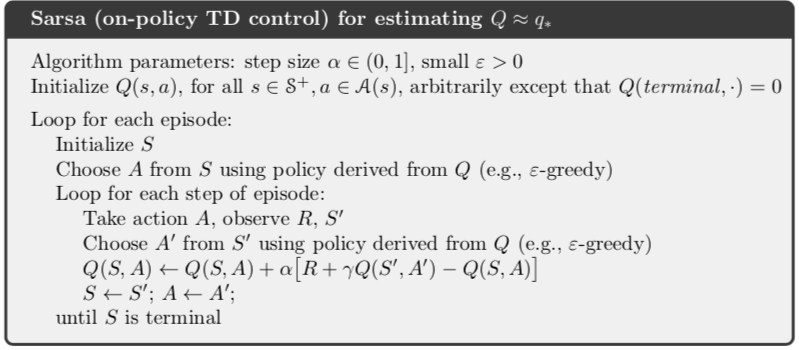
\includegraphics[width = \textwidth]{sarsa_algo}
  \caption{High level pseudocode description of sarsa algorithm for estimating $Q$}
\end{figure*}



\section{Related Work}
Reinforcement learning and deep reinforcement learning in particular have a history of success on fully observable games for Atari, such as Pong or Space Invaders \cite{playing_atari}. Most of the best performing AI solvers were trained using deep recurrent Q-learning, weighted replay, or dueling. Google DeepMind recently developed an Asynchronous Advantage Actor-Critic (A3C) model that has also been used to train AI solvers for Atari games with success as well. The victory of AlphaGo over the best human player received wide media attention as a landmark. While we restrict our focus in this project to deep-Q learning and SARSA, more complicated models have proven to be more successful especially running on more advanced architectures. 

Doom in particular has a history with using deep-Q networks to train solvers. Recent works on training the Doom AI have created models that outperform built-in bots and even some human players  


\section{Project Description}
We chose a very simple setting of the Doom game to train our agent. The setting for our project AI allows for the agent at any time step to do one of only three things: move left, right, or shoot. For each game episode, there is a stationary demon that does not attack the agent. Thus the goal for the 


\section{Experiments}
\subsection{Sarsa (on-policy TD control)}
To test the Sarsa algorithm on Doom, we needed to first tune the parameters of the experiment. Unfortunately it was determined that for significant learning to take place, large numbers of episodes (~20,000) needed to be performed. Consider the example in figures \ref{alpha1} and \ref{alpha2} of how Sarsa performed over 3000 trials for values of the learning rate alpha set to 0.1 and 0.2. It is clear that learning hardly takes place if at all for either learning rate. 

We decided to run the AI for a much larger number of episodes to see if we could witness learning taking place. We chose to do 120,000 episodes, where the $\epsilon-$greedy policy would anneal from $\epsilon = 1$, i.e. a completely random policy, to $\epsilon=0$, i.e. a greedy policy over the first 100,000 episodes. The last 20,000 episodes show the reward when the agent greedily followed the learned policy. Unfortunately the average reward is still negative, indicating that the policy learned still had much room for improvement. Nonetheless, it is still evident that average reward did increase and then level off when the policy became completely greedy. Thus it is reasonable to infer that with much more training, the agent could learn a successful policy, albeit slowly. 




\begin{figure}
\label{alpha1}
  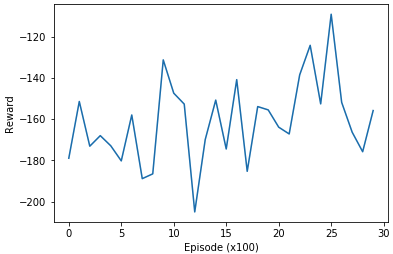
\includegraphics[width = \columnwidth]{sarsa_3k_alpha1}
  \caption{Running 120000 episodes of Sarsa with a smoothing window of 100 episodes. Learning rate was set to 0.1, $\epsilon$-greedy policy selection was used with annealing steps from 1 to 0 over 2500 episodes and the last 500 episodes follow a completely greedy policy }
\end{figure}

\begin{figure}
\label{alpha2}
  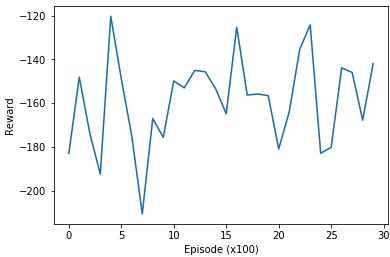
\includegraphics[width = \columnwidth]{sarsa_3k_alpha2}
  \caption{Running 3000 episodes of Sarsa with a smoothing window of 100 episodes. Learning rate was set to 0.2, $\epsilon$-greedy policy selection was used with annealing steps from 1 to 0 over 2500 episodes and the last 500 episodes follow a completely greedy policy }
\end{figure}


\begin{figure}
\label{100k}
  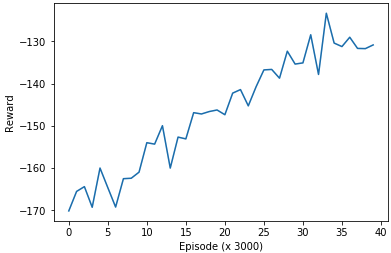
\includegraphics[width = \columnwidth]{sarsa_120k_3kwindow}
  \caption{Running 120000 episodes of Sarsa with a smoothing window of 1000 episodes. Learning rate was set to 0.1, $\epsilon$-greedy policy selection was used with annealing steps from 1 to 0 over 100000 episodes and the last 20000 episodes follow a completely greedy policy }
\end{figure}


\subsection{Deep-Q Learning}



\section{Conclusion}

\medskip
\printbibliography

















\end{document}